\chapter{Dettagli implementativi}
In questa sezione vedremo i dettagli implementativi di alcune parti pi\`u significative o complesse del sistema.

\section{RabbitMQ}
All'interno dell'architettura event-driven di Sentinel, il Credit Manager ha il ruolo di consumer.
Sono presenti tre Topic Exchange:
\begin{itemize}
  \item \textbf{work-exchange} - L'exchange dove vengono inviati i messaggi normalmente.
  \item \textbf{retry-exchange} - L'exchange dove vengono inviati i messaggi che hanno superato il numero massimo di retry nel work-exchange.
    Su questi messaggi viene applicato un exponential backoff, e se superano il numero massimo di retry anche qui vengono inviati nell'error-exchange. I messaggi in questo
    exchange hanno un TTL di 12000 (12 secondi).
  \item \textbf{error-exchange}- L'exchange dove vengono inviati i messaggi che hanno restituito un errore irrecuperabile o che hanno superato il numero massimo di retry.
\end{itemize}
\textbf{}\\
Il Credit Manager sta in ascolto sulla coda con topic ``\#.event.payment.\#'' del work-exchange, e riceve messaggi con il seguente formato:

\begin{lstlisting}[language=Java]
public class PaymentMessage {
  private UUID idempotencyKey;
  private PaymentOperationType operationType;
  private Money costFeedback;
  private long workflowId;
}
\end{lstlisting}
Di seguito la spiegazione della funzione di ogni campo:
\begin{itemize}
  \item \textbf{idempotencyKey} - UUID che verr\`a utilizzato come chiave primaria del nuovo movimento. Permette di evitare l'inserimento
    di operazioni duplicate.
  \item \textbf{paymentOperationType} - Contiene il Tipo Operazione, equivalente a quello salvato nel database. Viene utilizzato per recuperare il costo da addebitare
    al tenant dal listino prezzi associato.
  \item \textbf{costFeedback} - \`E il costo reale affrontato durante l'interrogazione alla banca dati esterna. Viene registrato in caso sia differente dal costo reale
  \item \textbf{workflowId} - \`E l'id del workflow, e viene utilizzato da alcuni endpoint per restituire statistiche come il totale speso in un determinato workflow.
\end{itemize}
Quando il Credit Manager riceve un messaggio sulla sua coda, registra il movimento nella tabella Movimento del database.

\section{Stripe}
Per l'implementazione di Stripe, \`e stato deciso di utilizzare il Checkout di Stripe con pagina self-hosted, in modo da integrare la pagina di Stripe all'interno
dell'applicativo. Un pagamento segue un flusso ben preciso:
\begin{figure}[H]
  \centering
  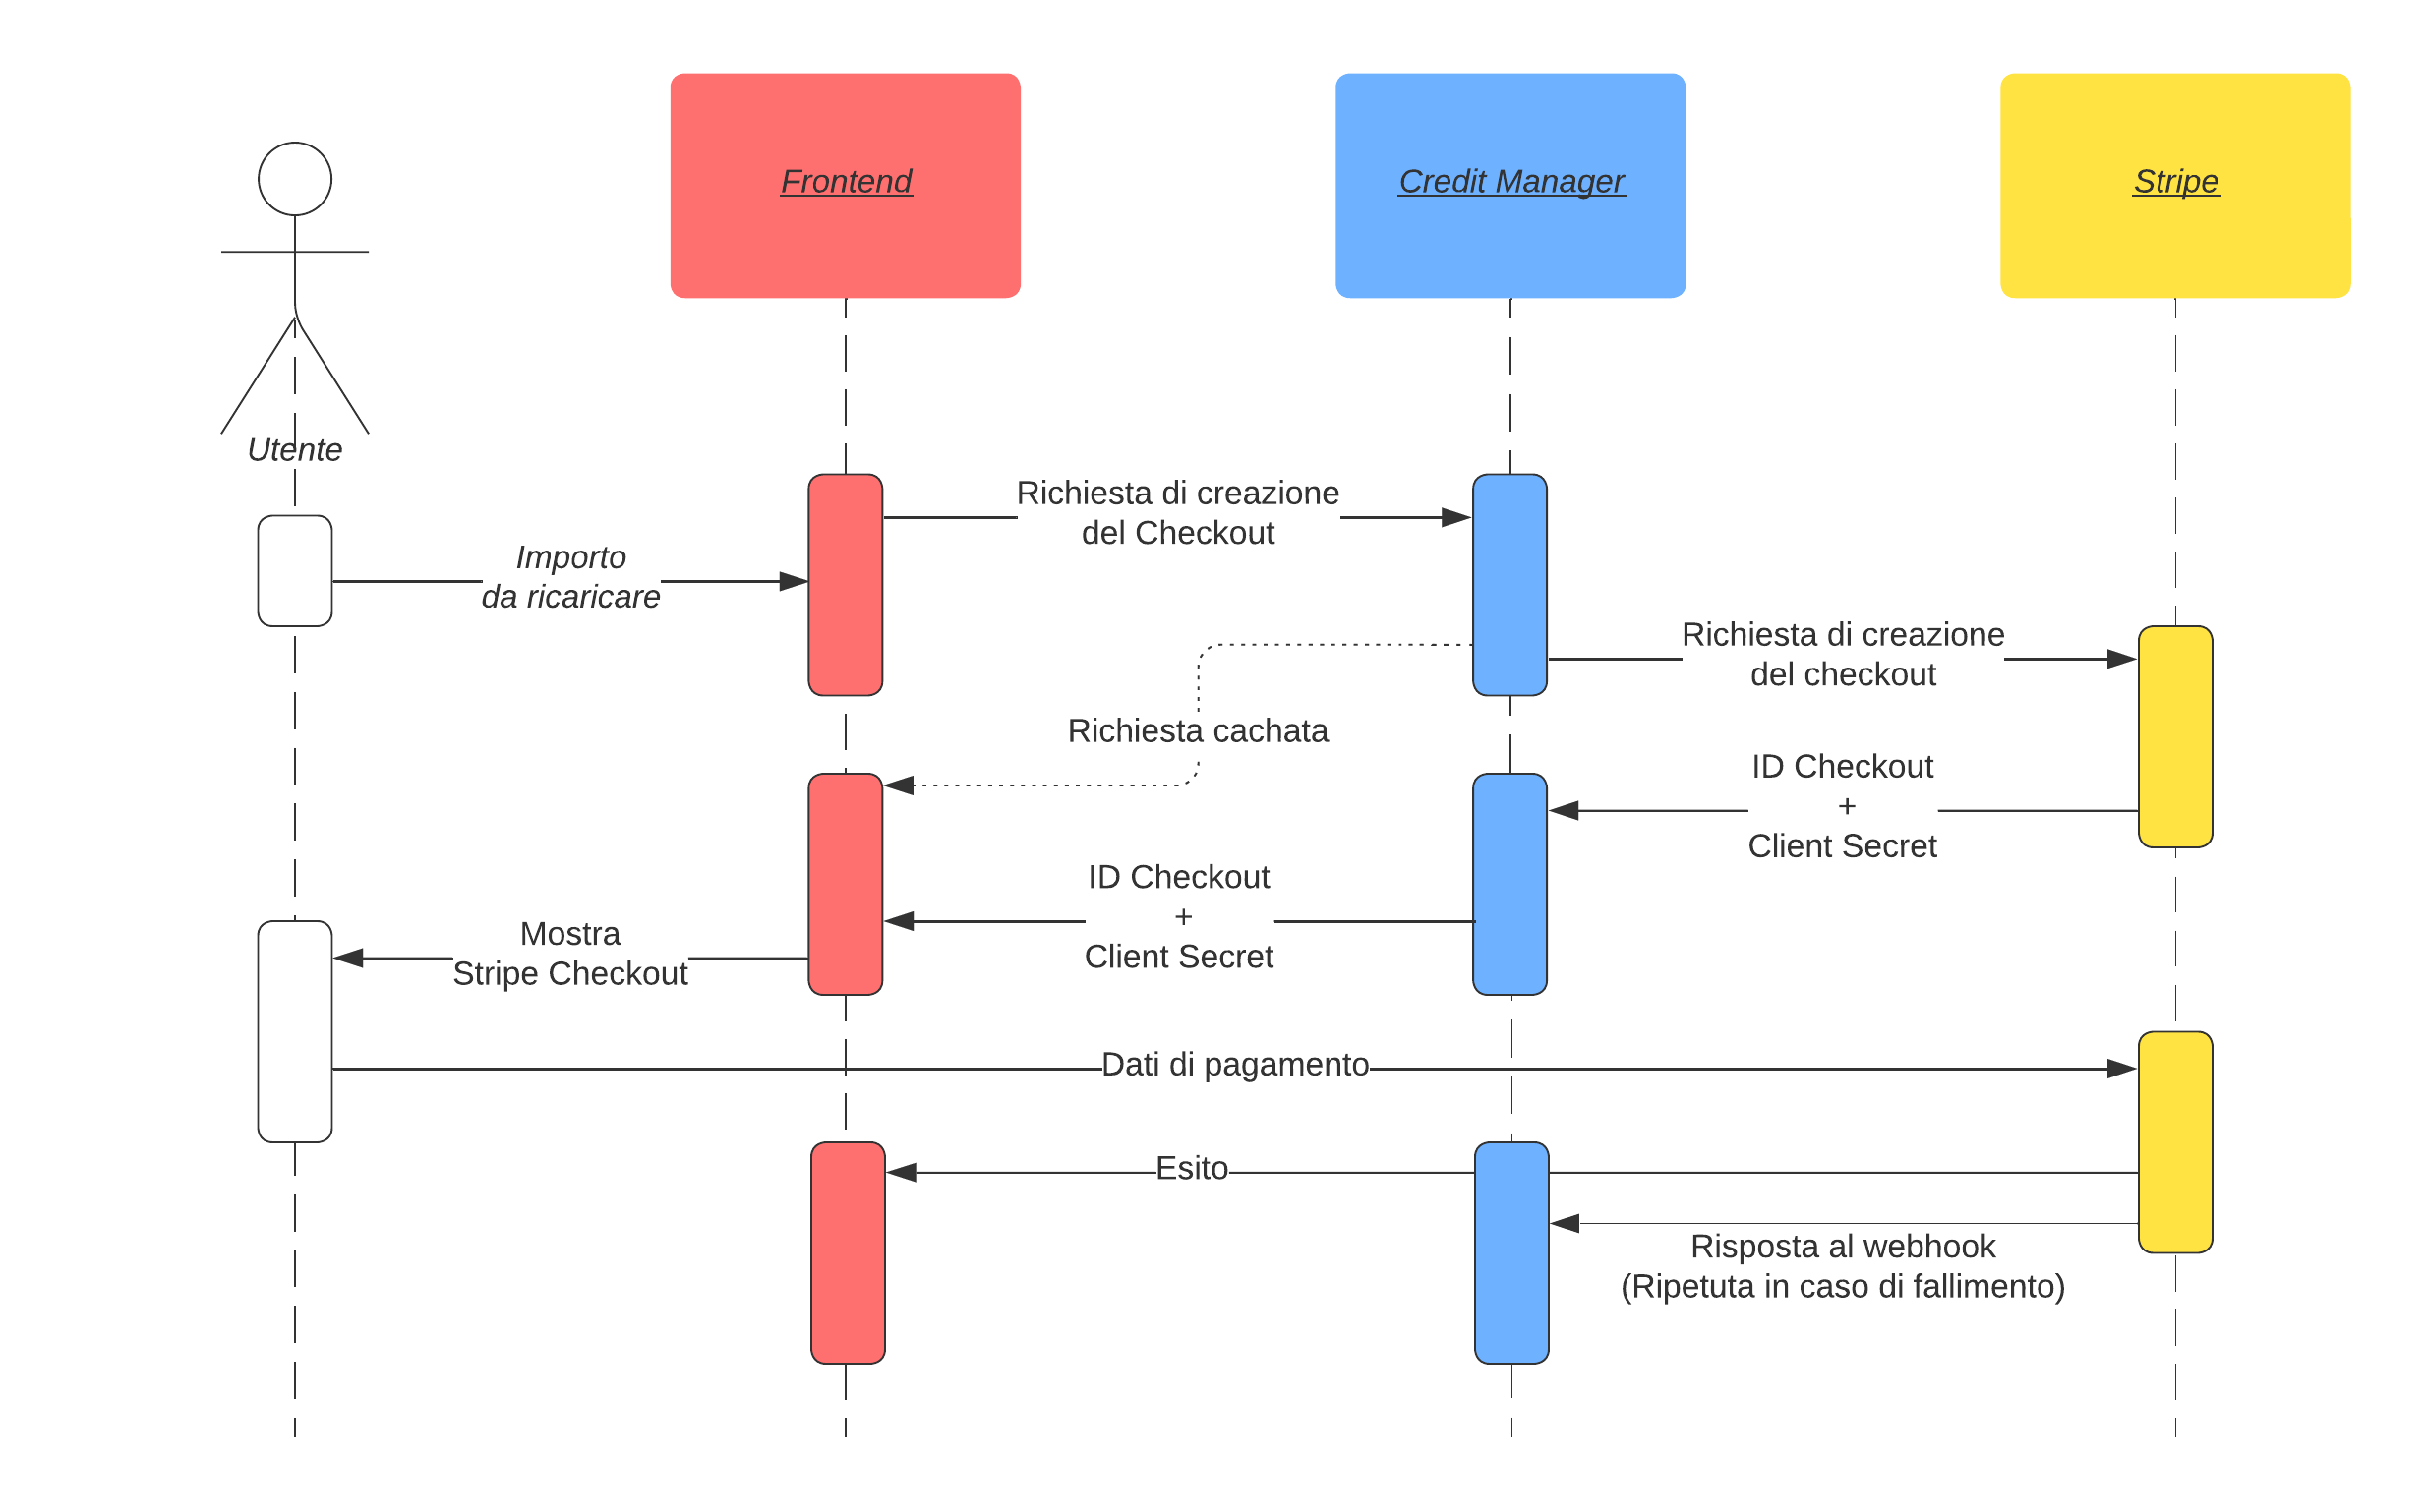
\includegraphics[width=14cm]{images/stripe-pagamento-diagramma.png}
  \caption{Diagramma di sequenza di un pagamento con Stripe}
  \label{stripepayment}
\end{figure}

\begin{enumerate}
  \item L'utente inserisce un importo maggiore di 5 euro da ricaricare e conferma.
  \item Il frontend invia l'importo con una chiave di idempotenza generata tramite UUID.
  \item Il backend verifica che la richiesta non sia gi\`a stata eseguita confrontandolo con la cache salvata su Redis, e nel caso invia al frontend la risposta precedente. In caso negativo invia a Stripe una richiesta di
    creazione del checkout con la stessa chiave di idempotenza inviata dal backend.
  \item Stripe risponde al backend con l'id del Checkout e un Client Secret necessario per creare il Checkout.
  \item Il backend risponde al frontend con le informazioni inviate da Stripe.
  \item Il frontend mostra il Checkout all'utente, utilizzando i dati inviati da Stripe.
  \item L'utente inserisce i dati di pagamento e li invia a Stripe attraverso l'elemento hostato da Stripe.
  \item Stripe invia l'esito sia al backend che al frontend. Nel caso del backend, l'esito viene inviato ad un webhook che si occupa di registrare correttamente l'avvenuto
    pagamento. In caso il backend non restituisca il codice HTTP 200 OK, Stripe riprover\`a fino a tre giorni seguendo una strategia di Exponential Backoff.
\end{enumerate}
\textbf{}\\
Il webhook ha il compito di verificare che i messaggi siano realmente provenienti da Stripe, confrontando la signature ricevuta nell'header ``Stripe-Signature'' con la
chiave ricevuta da Stripe durante la configurazione.

\section{SignalStore di NgRx}
Nel corso del tirocinio, l'azienda ha preso una decisione importante: ricostruire completamente il frontend a partire da una base diversa, utilizzando l'ultima
versione di Angular (Angular 17). Per questo fine, \`e stato deciso di rivedere il pattern di comunicazione tra componenti. In precedenza veniva utilizzato \textbf{NgRx}, un
progetto che porta il pattern Redux su Angular.

Viene quindi scelto di scommettere sul \textbf{SignalStore di NgRx}, interamente basato sui Signal usciti dalla Developer Preview proprio con la versione 17 di Angular.

Durante il tirocinio mi sono quindi occupato anche di implementare una soluzione flessibile che utilizzi al meglio il SignalStore.
\`E stato necessario implementare quelle che NgRx chiama \textbf{feature}, sfruttando al 100\% tutte le funzionalit\`a di TypeScript per evitare di compromettere la Type Safety.
Viene fatto uso di Generics, Mapped Types, Function Overloading, e viene in generale sfruttata la capacit\`a di inferenza sui tipi di TypeScript.
Le feature implementate offrono la possibilit\`a di effettuare operazioni \textbf{CRUD} (Create, Read, Update, Delete), ma rimuovono la necessit\`a di scrivere molto boilerplate e offrono funzionalit\`a aggiuntive.
\\\\
Ne sono state implementate tre:
\begin{itemize}
  \item \textbf{withItem}: Si occupa di effettuare operazioni CRUD su un singolo oggetto appartenente a una collezione.
  \item \textbf{withList}: Si occupa di effettuare operazioni CRUD su una collezione.
  \item \textbf{withGrid}: Si occupa di gestire lo stato necessario per un componente generico che mostra una Tabella. Permette inoltre di effettuare operazioni CRUD sulle righe
    della tabella.
\end{itemize}

Prenderemo in esame withGrid, la pi\`u complessa.
\\
\begin{lstlisting}
export const Store = signalStore(
    withGrid({
        collection: 'nomeCollezione',
        service: StoreService,
        paginationType: 'none',
        idField: 'id',
        defaultSorting: { dir: 'asc', field: 'createdTime' },
        usedInputs: ['form', 'routeParams', 'queryParams'],
    })
)
\end{lstlisting}
\textbf{}\\
Questo \`e il codice richiesto per creare uno Store che include withGrid. La feature prende in input diversi parametri:
\begin{itemize}
  \item \textbf{collection} - Il nome su cui verranno basati i nomi delle funzioni CRUD e dello stato.
  \item \textbf{service} - Oggetto che contiene i metodi che comunicano con il backend. Restituiscono
    l'\textbf{Observable}\footnote{Un Observable \`e la base della reattivit\`a fornita da RxJs: \`e una sorgente di dati che vengono emessi nel tempo.
      Il flusso pu\`o essere manipolato appendendo degli operatori che modificano il dato ad ogni passo. I pi\`u comuni sono map e filter.
    Angular li utilizza per le chiamate HTTP, e in questo caso emettono un valore una sola volta per subscription.}
    a cui lo store si sottoscriver\`a
    per effettuare la chiamata. \`E stato disposto un tipo generico che prende in input i tipi per definire i parametri necessari per le chiamate, tra cui il tipo
    dell'oggetto che lo Store deve gestire, o i routeParams che deve utilizzare per generare l'URL. Questo tipo generico consente a IDE moderni come Visual Studio Code di
    generare tutte le funzioni che poi verranno chiamate dalla feature.
  \item \textbf{paginationType} - Il tipo di paginazione utilizzato. Ha tre possibili valori: \textbf{none}, \textbf{blocks}, \textbf{pages}. Questo perch\`e lo store
    gestisce anche la paginazione per il componente generico, e si deve comportare in maniera diversa a seconda del tipo. Per blocks, la paginazione e il sorting
    vengono gestiti dal backend, che prende in input anche la dimensione del block e il numero di blocco. Nel caso di pages, invece, la paginazione \`e interamente gestita
    dalla feature e dal componente generico. Se il valore di paginationType \`e none viene disabilitata la paginazione.
  \item \textbf{idField} - Nome del campo ID dell'oggetto che la grid sta trattando. Il valore di questo campo deve essere necessariamente univoco negli oggetti inseriti,
    in quanto necessario per il corretto funzionamento della feature e del componente generico (per esempio, viene utilizzato nel track del @for di Angular).
  \item \textbf{defaultSorting} - Valore iniziale del campo per cui vengono ordinati gli oggetti all'interno della grid. Nella paginazione a blocchi questo valore viene inviato
    anche al backend, altrimenti viene utilizzato localmente.
  \item \textbf{usedInputs} - Valore utilizzato internamente dalla feature per abilitare o disabilitare determinati input. Il suo valore viene forzato attraverso il typing system
    di TypeScript utilizzando il tipo di Service.
\end{itemize}
\textbf{}\\
La feature mette a disposizione diverse funzioni e valori: tutte le tipiche funzioni CRUD, una funzione per effettuare il reload della grid con gli ultimi input passati,
e lo stato dell'ultima chiamata effettuata (Loading, Loaded, Error, o Init se non \`e stata effettuata nessuna chiamata dalla creazione dello store).
